
A continuous probability distribution has rather than discrete values   Trying to long tail and narrow while maintaing a constant mean. The gamma distribution fulfills these criteria.

Here we consider a slight modification to the traditional gamma distribution in the form of a truncated version. Let $\alpha, \beta > 0$. A random variable $X$ follows the truncated gamma distribution $\Gamma^T(\alpha, \beta)$ if it has the probability density function 
%
\begin{align}
  f_{\alpha,\beta}(x) = \begin{cases} K_{\alpha, \beta}\,
\frac{1}{\beta^{\alpha}\Gamma(\alpha)}\, x^{\alpha-1}\,e^{-x/\beta} & 0 \leq x \leq 1 \\
0 & \text{otherwise}.
\end{cases}
\end{align}
%
The factor $K_{\alpha,\beta}$ is needed due to the truncation of the probability density function for $x>0$ to ensure that
\begin{align}
  \int f_{\alpha,\beta}(x) \,dx = 1. \label{eq:gd1}
\end{align}
The value of $K_{\alpha,\beta}$ is the inverse of the cumulative probability $x \leq 1$ of the untruncated gamma distribution,
\begin{align}
  K_{\alpha,\beta} = \left(\int_0^{1} \frac{1}{\beta^{\alpha}\Gamma(\alpha)}\, x^{\alpha-1}\,e^{-x/\beta} \, dx \right)^{-1}.
\end{align}
With this the equality~\eqref{eq:gd1} clearly holds. Consider then the above network model in which the connection probabilities $P_{ij}$ are $\Gamma^T(\alpha, \beta)$ distributed. As $K_{\alpha,\beta}$ is a constant for fixed $\alpha$ and $\beta$, many results on the standard gamma distribution can be adapted to the truncated version by multiplication with $K_{\alpha,\beta}$. We note the following results for the overall connection probability $\mu$,
%
\begin{align}
 \mu = \E(P_{ij}) = K_{\alpha,\beta} \, \alpha \beta, \label{eq:gd1}
\end{align}
and the expected occurrence of bidirectional connections
\begin{align}
  \E(P_{ij}^2) = K_{\alpha,\beta} \, (\alpha^2 \beta^2 + \alpha \beta^2).
\end{align}
%
The overrepresentation is then
\begin{align}
  \sigma & = \frac{\E(P_{ij}^2)}{\E(P_{ij})^2} =% \frac{\alpha^2 \beta^2}{\alpha^2 \beta^2} + \frac{\alpha \beta^2}{\alpha^2 \beta^2} =
 \frac{1}{K_{\alpha,\beta}} \left(1 + \frac{1}{\alpha}\right).
\end{align}

\begin{figure}[h!]
\centering
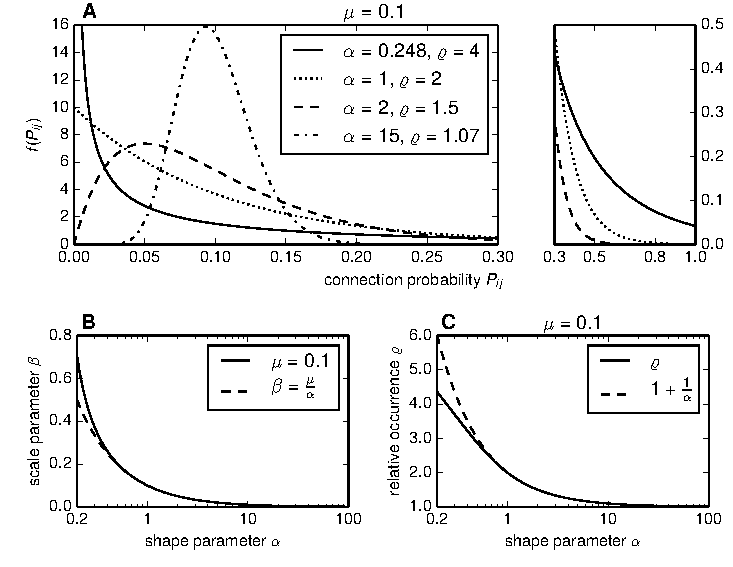
\includegraphics[width=0.703\textwidth]{../lab/gamma_distribution/gamma_figure.png}
\includegraphics[width=0.287\textwidth]{../lab/gamma_distribution/gamma_figure_logscale.png}
\caption{Probability density functions of the truncated gamma distribution for different shape parameters $\alpha$ and the induced relative overrepresentation of bidirectional connections $\sigma$ in a network with such distributed connection probabilities $P_{ij}$. For given $\alpha$ the parameter $\beta$ was estimated numerically to yield $\mu \approx 0.1$ in all distributions shown.}
\label{fig:gd}
\end{figure}

In Figure~\ref{fig:gd} probability density functions for multiple parameter sets $(\alpha, \beta)$ are shown. The rate parameter $\beta$ is determined by the given $\alpha$ and $\mu = 0.1$ through the relation in \eqref{eq:gd1}. [Comment: I'm not sure it's worth deriving an expression for $\beta$. A good approximation is $\beta = \frac{\mu}{\alpha}$, ($K_{\alpha,\beta} = 1$). I just need to make it clear what I'm doing.]
The narrower the probability density around the mean $\mu = 0.1$ the smaller is the expected overrepresentation of bidirectional connections $\sigma$ in the network. To achieve a high $\sigma$ many pairs with a high connection probability are needed. The dashed line in Figure~\ref{fig:gd} marks the probability density function of the probability distribution of connection probabilities $P_{ij}$ that induce an overrepresentation of reciprocal pairs of $\sigma = 4$ as found by \textcite{Song2005} leading to a highly skewed distribution with a long tail. The relevance of such a distribution for cortical networks however is debatable, as most connections are with a high certainty not established seemingly wasting the network's potential for different possible configurations.





%References: \href{http://herbsusmann.com/distributions/gamma-distribution-variance-proof.html}{Proof $\E(X^2)$}, 

